\begin{activity} \label{A:11.7.6} A solid $S$ is bounded below by the square $z=0$, $-1 \leq x \leq 1$, $-1 \leq y \leq 1$ and above by the surface $z = 2-x^2-y^2$. A picture of the solid is shown in Figure \ref{F:11.7.COM3D}.
\begin{figure}[ht]
\begin{center}
%\resizebox{!}{2.0in}{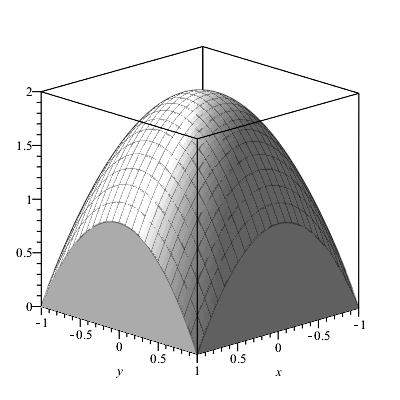
\includegraphics[trim=0cm 0.5cm 0cm 1cm, clip]{11_7_COM3D}}
  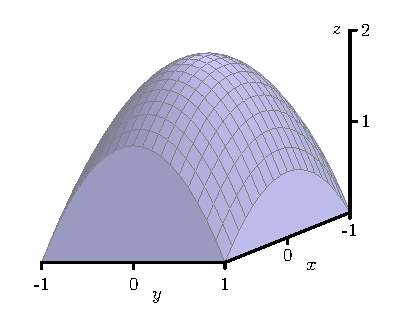
\includegraphics{figures/fig_11_7_volume.eps}
\end{center}
\caption{The solid bounded by the surface $z = 2-x^2-y^2$.}
\label{F:11.7.COM3D}
\end{figure}
%crop graphics in animate trim=<left> <bottom> <right> <top>, clip with includegraphics

    \ba
    \item Set up (but do not evaluate) an iterated integral to find the volume of the solid $S$.

    \item Set up (but do not evaluate) iterated integral expressions that will tell us the center of mass of $S$, if the density at point $(x,y,z)$ is $\delta(x,y,z)=x^2+1$.

    \item Set up (but do not evaluate) an iterated integral to find the average density on $S$ using the density function from part (b).

    \item Use technology appropriately to evaluate the iterated integrals you determined in (a), (b), and (c); does the location you determined for the center of mass make sense?

    \ea

\end{activity}
\begin{smallhint}

\end{smallhint}
\begin{bighint}

\end{bighint}
\begin{activitySolution}
    \ba
    \item We integrate first with respect to $z$, so that $0 \leq z \leq 2-x^2-y^2$. The projection of the surface onto the $xy$-plane is the square, so an iterated integral that gives the volume of $S$ is 
\[\int_{-1}^1 \int_{-1}^1 \int_0^{2-x^2-y^2} dz \, dy \, dx.\]

    \item The center of mass of $S$ is $(\overline{x}, \overline{y}, \overline{z})$, where 
\begin{align*}
\overline{x} &= \frac{\int_{-1}^1 \int_{-1}^1 \int_0^{2-x^2-y^2} x(x^2+1) \, dz \, dy \, dx}{\int_{-1}^1 \int_{-1}^1 \int_0^{2-x^2-y^2} x^2+1 \, dz \, dy \, dx} \\
\overline{y} &= \frac{\int_{-1}^1 \int_{-1}^1 \int_0^{2-x^2-y^2} y(x^2+1) \, dz \, dy \, dx}{\int_{-1}^1 \int_{-1}^1 \int_0^{2-x^2-y^2} x^2+1 \, dz \, dy \, dx} \\
\overline{z} &= \frac{\int_{-1}^1 \int_{-1}^1 \int_0^{2-x^2-y^2} z(x^2+1) \, dz \, dy \, dx}{\int_{-1}^1 \int_{-1}^1 \int_0^{2-x^2-y^2} x^2+1 \, dz \, dy \, dx}.
\end{align*}

    \item The average density is given by 
\[\frac{\int_{-1}^1 \int_{-1}^1 \int_0^{2-x^2-y^2} x^2+1 \, dz \, dy \, dx}{\int_{-1}^1 \int_{-1}^1 \int_0^{2-x^2-y^2} 1 \, dz \, dy \, dx}.\]

	\item The volume of the solid is $\frac{16}{3}$, the center of mass is $\left(0,0,\frac{94}{133}\right)$, and the average density is $\frac{19}{15}$. Given the symmetry, we should expect $\overline{x}$ and $\overline{y}$ to be 0. Since the bulk of the mass is nearer to the $xy$-plane, it makes sense that $\overline{z}$ is less than 1.  
    \ea
\end{activitySolution}
\aftera
